\documentclass{article}

\usepackage[french]{babel}
\usepackage[utf8]{inputenc}
\usepackage{amsmath}
\usepackage{graphicx}
\usepackage{subcaption}
\usepackage[colorlinks=true, allcolors=blue]{hyperref}


%%%%%%%%%%%%%%%% Lengths %%%%%%%%%%%%%%%%
\setlength{\textwidth}{15.5cm}
\setlength{\evensidemargin}{0.5cm}
\setlength{\oddsidemargin}{0.5cm}

%%%%%%%%%%%%%%%% Variables %%%%%%%%%%%%%%%%
\def\projet{6}
\def\titre{Résolution approchée d'équations différentielles / Modélisation de systèmes dynamiques }
\def\groupe{1}
\def\equipe{3}
\def\responsible{qchavignytu}
\def\secretary{mbouhaja}
\def\others{ lperrin011, alagraoui001}

\begin{document}

%%%%%%%%%%%%%%%% Header %%%%%%%%%%%%%%%%
\noindent\begin{minipage}{0.98\textwidth}
  \vskip 0mm
  \noindent
  { \begin{tabular}{p{7.5cm}}
      {\bfseries \sffamily
        Projet \projet} \\ 
      {\itshape \titre}
    \end{tabular}}
  \hfill 
  \fbox{\begin{tabular}{l}
      {~\hfill \bfseries \sffamily Groupe \groupe\ - Equipe \equipe
        \hfill~} \\[2mm] 
      Responsable : \responsible \\
      Secrétaire : \secretary \\
      Codeurs : \others
    \end{tabular}}
  \vskip 4mm ~

  ~~~\parbox{0.95\textwidth}{\small \textit{Résumé~:} \sffamily Ce projet se concentre sur les méthodes de résolution d'équations différentielles ordinaires (EDO) et explore leur vitesse de convergence et leur précision.  }
  \vskip 1mm ~
\end{minipage}

%%%%%%%%%%%%%%%% Main part %%%%%%%%%%%%%%%%
\section{Résolution d'équations différentielles }

\textbf{Bouhaja Mohammed}

Dans cette partie, nous allons programmer différentes méthodes numériques de résolution des équations différentielles. Ces méthodes sont basées sur des algorithmes à un pas (1), où chaque étape de la résolution est calculée en fonction de l'étape précédente. 

\begin{equation}
    y_{n+1} = y_{n}+h_{n}*\Phi(y_{n}, t_{n}, h_{n})
\end{equation}

% L'objectif est de représenter un problème de Cauchy de manière unifiée en utilisant une représentation adaptée pour la condition initiale et la fonction différentielle de l'équation. Cette représentation doit être capable de gérer des équations différentielles de dimension arbitraire.

Ensuite, nous implémentons deux autres fonctions. La première de ces deux fonctions permet d'obtenir le résultat après un nombre donné $n$ d'itérations. La deuxième fonction permet d'obtenir le résultat en fonction d'une précision donnée $eps$.

\subsection{Comparaison des solutions obtenues par différentes méthodes de calcul}
Afin de vérifier la précision des méthodes de résolution que nous avons implémentées, nous avons considéré une équation différentielle du premier ordre. Nous avons calculé la solution de cette équation en utilisant les différentes méthodes (Euler, point milieu, Heun et Runge-Kutta d'ordre 4). Ensuite, nous avons comparé les résultats obtenus pour s'assurer de leur cohérence.

\begin{figure}[h]
    \begin{minipage}[c]{.4\linewidth}
        \includegraphics[width=7cm]{img/all_sol.png}
        \caption{Les différentes méthodes comparées à la solution exacte}
        \label{fig:all}   
    \end{minipage}
    \hfill
    \begin{minipage}[c]{.4\linewidth}
        \includegraphics[width=7cm]{img/convergence.png}
        \caption{La convergence des quatre méthodes.}
        \label{fig:conv}
    \end{minipage}
\end{figure}

Ensuite on s'intéresse à la vitesse de convergence de chaque méthode.


La méthode d'Euler a une convergence linéaire, ce qui la rend relativement lente pour atteindre une précision élevée. La méthode du point milieu et la méthode de Heun offrent une convergence quadratique, convergeant plus rapidement et fournissant une meilleure précision que la méthode d'Euler. La méthode de Runge-Kutta d'ordre 4 est la plus précise des quatre méthodes, offrant une convergence exponentielle et une grande précision dans la résolution des équations différentielles.

\subsection{Le champ des tangentes de l’équation différentielle}

\begin{figure}[h]
    \centering
    \includegraphics[scale=0.4]{img/champ_tang.png}
    \caption{ champ des tangentes de l'équation différentielle $y'(x,y)=x^{2}+y^{2}$.}
    \label{fig:champ}
\end{figure}

En utilisant la fonction "quiver" pour dessiner le champ des tangentes d'une équation différentielle de dimension 2, nous obtenons un graphique qui représente visuellement la direction et la magnitude des vecteurs tangents en différents points du plan. Ce champ de tangentes offre une représentation graphique intuitive du comportement des solutions de l'équation différentielle, permettant de visualiser les trajectoires.

\subsection{Tests pour les deux équations différentielles\\}

En utilisant les méthodes de résolution numérique que nous avons implémentées, nous cherchons à obtenir des approximations des solutions pour les équations différentielles en dimension 1 et 2.


\paragraph{En dimension 1}
\begin{equation}
\begin{cases}
\begin{aligned}
    y(0) = 1 \\
    y'(t) = \frac{y}{1+t^{2}}  
\end{aligned}
\end{cases}
\end{equation}




\paragraph{En dimension 2}

\begin{equation}
\begin{cases}
\begin{aligned}
y(0) &= \begin{bmatrix} 0 \\ 1 \end{bmatrix}\\
y'(t) &= \begin{bmatrix} -y_{2}(t) \\ y_{1}(t) \end{bmatrix} 
\end{aligned}
\end{cases}
\end{equation}


\begin{figure}[h]
    \centering
    \begin{subfigure}{0.44\textwidth}
        \centering
        \includegraphics[scale=0.3]{img/sol_dim1.png}
       \caption{La solution en dimension 1}
        \label{fig:dim1}
    \end{subfigure}
    \begin{subfigure}{0.44\textwidth}
        \centering
    \includegraphics[scale=0.3]{img/sol_dim_2.png}
    \caption{La solution en dimension 2}
    \label{fig:dim2}
    \end{subfigure}
    \caption{la solution des deux équations différentielles (1) et (2) par les quatre méthodes.}
    \label{fig:ensemble}
\end{figure}

Les méthodes numériques de résolution d'équations différentielles fournissent des approximations de la solution réelle avec des erreurs liées à l'approximation des dérivées et à la non-linéarité des fonctions vu que la solution de la première équation différentielle est $x\longrightarrow exp(arctan(x))$ et de la deuxième équation $y_{1}(t)=cos(t)$ et $y_{2}(t)=sin(t)$. Les méthodes d'ordre supérieur, comme la méthode de Runge-Kutta d'ordre 4, offrent généralement des approximations plus précises. L'erreur de troncature peut être réduite en diminuant la taille du pas de temps. Il est important de comparer les résultats avec des solutions analytiques pour évaluer leur précision.

\section{Applications}
Grâce à ces méthodes de résolution, il est possible de s'intéresser à différents problèmes scientifiques.

\subsection{Modélisation du problème à trois corps}
Le problème des trois corps est un problème classique de la mécanique céleste qui consiste à prédire les mouvements de trois corps en interaction gravitationnelle mutuelle. Ce problème est important car il permet de modéliser de nombreux phénomènes astronomiques tels que les mouvements des planètes, des étoiles binaires, et même des galaxies. Dans cette partie, on s'intéresse à la résolution d'équations différentielles qui régissent ce système avec les méthodes implémentées précédemment. 

\subsubsection{Interactions gravitationnelles entre deux astres}
Au départ, on cherche à modéliser les interactions gravitationnelles entre deux corps massifs ponctuels $A$ et $B$ placés dans un plan, en considérant que chaque corps est soumis uniquement à la force d'interaction gravitationnelle engendrée par l'autre corps.

Afin de simplifier le problème, on suppose que la masse du corps $B$ est très faible devant celle de $A$. Plus formellement, on a $m_{A} \gg m_{B}$. Cette simplification implique que le corps $A$ peut être supposé immobile et insensible à l’interaction gravitationnelle de $B$.
On considérera comme référentiel d'étude le référentiel cartésien d'origine le centre de gravité de $A$. En appliquant le $PFD$ sur le corps $B$ soumis à la force gravitationnelle appliquée par $A$, on obtient l'équation suivante:
\[ 
m_{B}\frac{d\overrightarrow v_{B}}{dt} = \overrightarrow{F}_{A\to B} = \frac{\mathbf{G} m_{A}m_{B} \overrightarrow{BA} }{||\overrightarrow{BA} ||^{3}} \]
En projetant cette équation suivant les axes $Ox$ et $Oy$ on obtient le système d'équations différentielles suivant:

\begin{equation}\label{eq4}
\left\{
\begin{aligned}
& \ddot x_{B}  = \frac{\mathbf{G} m_{A} (x_{A} - x_{B}) }{r_{AB}^{3}}\\
& \ddot y_{B}  = \frac{\mathbf{G} m_{A} (y_{A} - y_{B}) }{r_{AB}^{3}}
\end{aligned}
\right.
\end{equation}
avec $x_{B}, y_{B}$ les coordonnées du corps $B$ , $x_{A}, y_{A}$ celles de $A$ supposé fixe et $r_{AB}$ la distance entre $A$ et $B$ exprimée par cette relation : $r_{AB} = \sqrt{(x_{A} - x_{B})^{2} + (y_{A} - y_{B})^{2}}$.\\

Afin de résoudre analytiquement ce système couplé, on pose comme inconnu le vecteur $[x_{B},
y_{B}, \dot x_{B},\dot y_{B}]$. Ensuite, nous donnons la fonction $F$ suivante comme argument des méthodes de résolution implémentées : $F : [x_{B}, y_{B}, \dot x_{B},\dot y_{B}] \longrightarrow [\dot x_{B},\dot y_{B}, \ddot x_{B},\ddot y_{B}] $. Ensuite, il suffit de remplacer les dérivées secondes avec les formules de l'équation~\ref{eq4}.

\subsubsection{Résolution de l'équation de mouvement}
Les figures~\ref{fig:_fig1} et~\ref{fig:_fig2} montrent deux trajectoires du corps $B$ obtenues après la résolution de l'équation du mouvement par la méthode $Runge-Kutta$ avec une masse $A$ fixée à $100$ unités de masse. Sur la figure~\ref{fig:_fig1}, les positions initiales respectives de $A$ et $B$ sont $(1,0)$ et $(3,0)$. On remarque que $B$ a un mouvement elliptique autour de $A$. Pourtant, un mouvement circulaire de centre $A$ est attendu. 

En outre, pour l'exemple de la figure avec une position initiale de $B $ égale à $(1.3, 0)$, très proche de celle de $A$, on remarque que la trajectoire de $B$ est discontinue au voisinage de cette position initiale, et cela se remarque par la superposition de plusieurs ellipses au voisinage de ce point. Dans ce cas, le mouvement de $B$ n'est pas circulaire de centre $A$.
            \begin{figure}[h]
                \begin{minipage}[c]{.4\linewidth}
                    % \centering
                    \includegraphics[width = 10cm, height = 7cm]{img/project6_1.png}
                    % \vspace{0.1cm}
                    \caption{Trajectoire du corps B}
                    \label{fig:_fig1}
                \end{minipage}
            \hfill%
                \begin{minipage}[c]{.4\linewidth}
                      % \centering
                    \includegraphics[width = 7.5cm, height = 7cm]{img/projet6_2.png}
                    \caption{Trajectoire du corps B}
                    \label{fig:_fig2}
                \end{minipage} 
            \end{figure}

\subsubsection{ Introduction d'un troisième corps massif}
Ensuite, on introduit un autre astéroïde $C$ de masse $m_{C}$ telle que $m_{A} \gg m_{B} \gg m_{C}$. On considère que le centre de gravité du système est proche de celui de $A$, et que $B$ suit une trajectoire circulaire autour de $A$ de rayon $R_{AB} = ||\overrightarrow AB|| = 1$. Ainsi, par la troisième loi de $Kepler$, on peut extraire la valeur de la période d'évolution $T$:
\[\frac{T^2}{(R_{AB})^3} = \frac{4\pi^2}{G(m_{A}+m_{B})} \implies T = \sqrt{\frac{4\pi^2 R_{AB}^{3}}{G(m_{A}+m_{B})}}  \] 

Alors, les équations de mouvements de $B$ s'expriment en coordonnées cartésiennes, comme suit:
\begin{equation}\label{eq5}
\left\{
\begin{aligned}
& x_{B}(t) = R_{AB} cos(2\pi T) \\
&  y_{B}(t) = R_{AB} sin(2\pi T) 
\end{aligned}
\right.
\end{equation}

Pour le mouvement de $C$ peut être déterminée en réapplicant le $PFD$ à $C$ soumis à la force gravitaionnelle due à la présence de $A$ et $B$, le système différentiel qui régit ce mouvement est le suivant:


\begin{equation}\label{eq6}
\left\{
\begin{aligned}
& \ddot x_{C}  = \frac{\mathbf{G} m_{B} (x_{B} - x_{C}) }{r_{BC}^{3}} + \frac{\mathbf{G} m_{A} (x_{A} - x_{C}) }{r_{AC}^{3}} \\
& \ddot y_{C}  = \frac{\mathbf{G} m_{A} (y_{B} - y_{C}) }{r_{BC}^{3}} + \frac{\mathbf{G} m_{A} (x_{A} - x_{C}) }{r_{AC}^{3}}
\end{aligned}
\right.
\end{equation}\\


Comme les coordonnées de $B$ sont exprimées dans l'équation~\ref{eq5} et comme $A$ est supposé fixe, la résolution de ce système s'effectue de la même manière que dans le cas de deux corps. Pour les distances on les calcule de la même façon puisque on dispose des expression des coordonnées de tous les points.

Les figures~\ref{3corps1} et ~\ref{3corps2} montrent deux exemples de trajectoires de l'anthérozoïde C pendant son mouvement. Sur la figure~\ref{3corps1}, la position initiale de $C$ est $(5,2)$ ce qui donne une trajectoire presque circulaire mais de centre écarté du centre de gravité de $A$ tandis que $B$ garde son mouvement circulaire et cela est du au masses des deux astres qui sont largement différentes, ainsi l'action de $C$ sur $B$ est supposée négligeable.

Pourtant, sur la figure~\ref{3corps2}, on observe une trajectoire différente de $C$, en effet, il décrit un ensemble d'orbites et cela peut être expliqué soit par la position de départ qui est très proche de celle de $A$, ou par un non planéité du mouvement. Il est à noter que $B$ garde le même mouvement dans les deux cas sauf que les échelles des axes sur les deux figures se diffèrent.
            \begin{figure}[h]
                \begin{minipage}[c]{.4\linewidth}
                   \includegraphics[width = 8cm, height =6.5cm ]{img/projet6_3.png}
                    \caption{Trajectoire de l'astre C}
                    \label{3corps1}
                \end{minipage}
            \hfill%
                \begin{minipage}[c]{.4\linewidth}
                     \includegraphics[width = 10cm, height =6.5cm ]{img/projet6_4.png}
                    \caption{Trajectoire de l'astre C}
                    \label{3corps2}
                \end{minipage} 
            \end{figure}
\newpage
\subsubsection{ Changement de référentiel d'étude }
Comme le mouvement de B est connu, il est possible d’effectuer un changement de base après la fin du calcul (une rotation), de manière a ce que les corps A et B restent fixes. Il est alors possible de ne s’intéresser qu’aux mouvements du corps C.


Pour étudier le mouvement de la planète C par rapport aux planètes A et B, il est possible de fixer A et B en appliquant une rotation appropriée au référentiel de départ. Cela permet d'obtenir un nouveau référentiel dans lequel A et B sont fixes et la trajectoire de C peut être tracée. La rotation peut être déterminée en calculant le vecteur position de B par rapport à A et l'angle de rotation nécessaire pour fixer B dans le référentiel fixe. Ensuite, une matrice de rotation 2D peut être construite pour effectuer la rotation souhaitée et appliquée à chaque point de la trajectoire de C pour obtenir la trajectoire dans le nouveau référentiel.

la matrice de rotation qui permet de faire ces modifications au système est la matrice $R$ définie par:

\hspace{4cm} R = \begin{pmatrix}
cos(\theta) & -sin(\theta) \\
sin(\theta) & cos(\theta) 
\end{pmatrix}\\
avec $\theta = \frac{2\pi T_{0}}{T} = 2\pi T_{0}$ car le corps B est supposé en rotation circulaire autour du soleil, avec une période de $\2\pi$ jours terrestres, ici $T_{0}$ est la durée du mouvement de $B$.


\subsection{Réaction chimique oscillante}

 La majorité des réactions chimiques connues sont dites "stables", c'est-à-dire qu'au sein de celles-ci, il n'y a, à partir d'un certain temps, plus d'interaction entre les réactifs. En opposition, certaines réactions chimiques particulières sont qualifiées d'"oscillantes" car leurs comportements suivent un modèle périodique. 

Soit le système oscillant \eqref{sys_oscil} avec les constantes $a=10$, $c=200$, $b\in[0.1, 0.2]$, $d=50$ et comme conditions initiales $[1, 0, 0]$ :

\begin{equation}
\label{sys_oscil}
\left\{
\begin{aligned}
\frac{dX}{dt} &= a + bY - X - ZY^2 \\
\frac{dY}{dt} &= c(X + XY^2 - Y) \\
\frac{dZ}{dt} &= d(Y - Z) \\
\end{aligned}
\right.
\end{equation}

\begin{figure}[h]
    \centering
    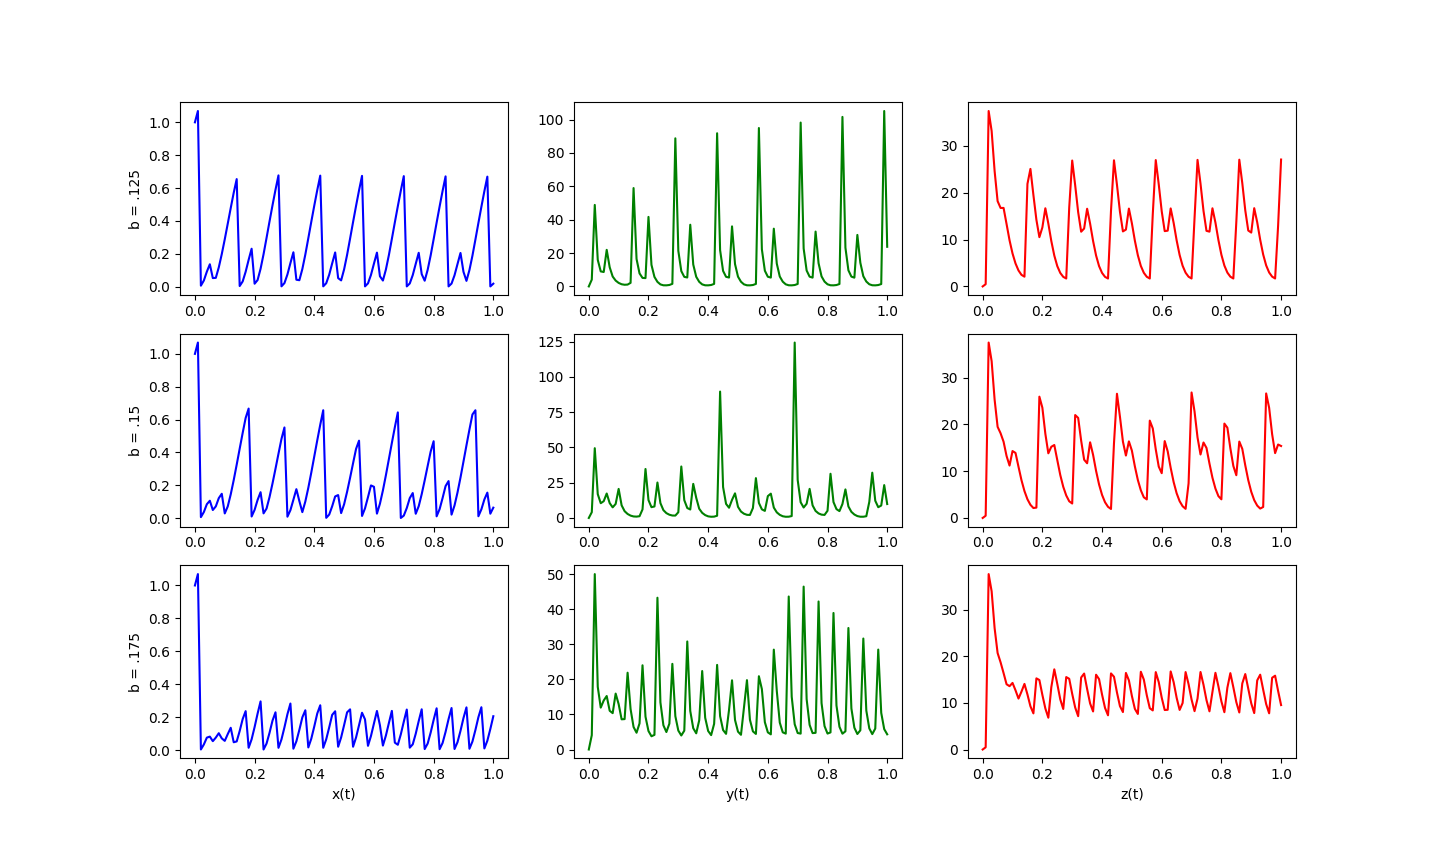
\includegraphics[width=13cm, height = 10cm]{img/graph_reac_chim_2.png}
    \caption{Représentation de X(t), Y(t) et Z(t) pour 3 valeurs de b différentes}
    \label{fig:grc2}
\end{figure}

Il est remarquable sur la figure \ref{fig:grc2} qu'une phase périodique se met en place pour les 3 valeurs de b vers $t=0.2$. \\

La notion de période d'un système correspond au nombre de maxima locaux de Y sur une période. Les travaux de Li et Yorke montrent une corrélation entre la période d'un système et le fait qu'il contienne des solutions chaotiques. \\

Soit la fonction retournant pour une valeur de b donnée l'ensemble des valeurs des maxima locaux de Y sur une période : il peut alors être tracé un nuage de points présentants pour de nombreuses valeurs de b les points de coordonnées (b, m), où m est la valeur d'un maximum local de Y.

\begin{figure}[h]
    \begin{minipage}[c]{.4\linewidth}
        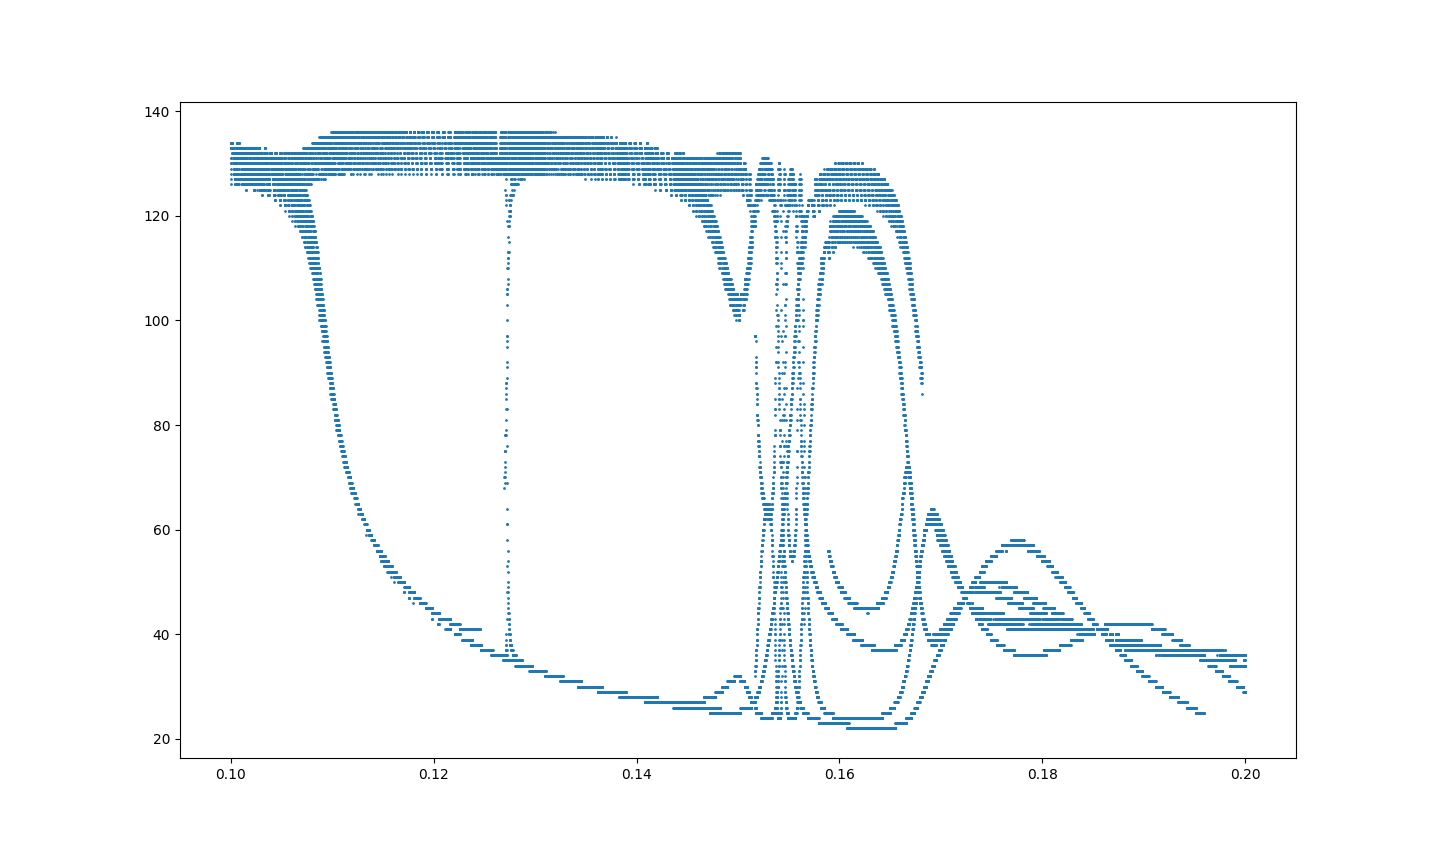
\includegraphics[width = 8cm]{img/graphe_b_y.png}
        \caption{Max. of Y depending on b}
        \label{fig:_by}
    \end{minipage}
        \hfill%
    \begin{minipage}[c]{.4\linewidth}
        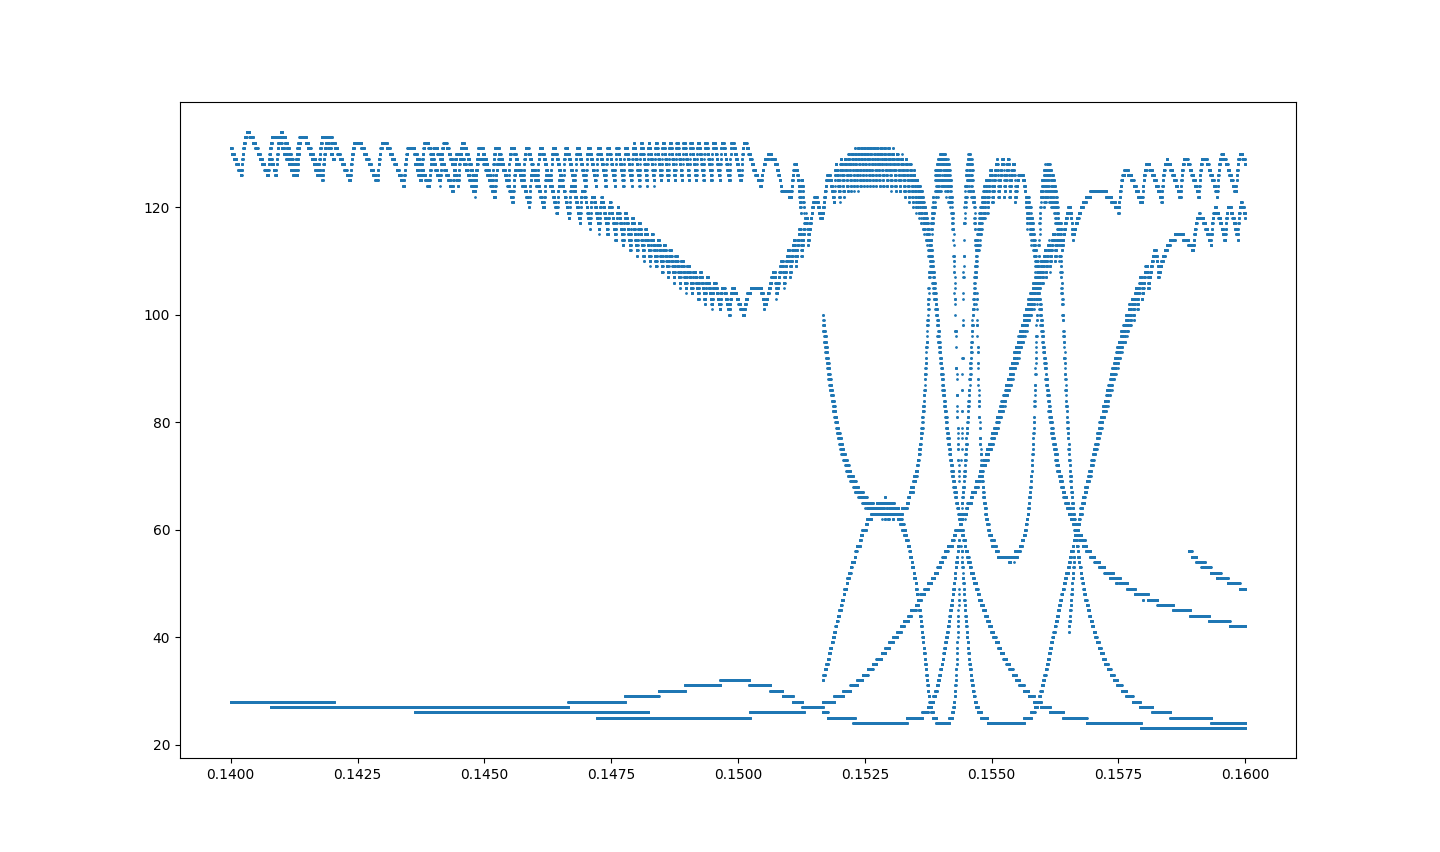
\includegraphics[width = 8cm]{img/graphe_b_y_14_16.png}
        \caption{Zoom on $b\in[0.14, 0.16]$}
        \label{fig:_by_14_16}
    \end{minipage} 
\end{figure}

Il a été difficile d'isoler une unique période de Y car les amplitudes des maxima diffèrent d'une période à l'autre et d'une valeur de b à l'autre. Sur les figures \ref{fig:_by} et \ref{fig:_by_14_16} tous les maxima locaux sont représentés par soucis de simplicité, car le fait de rajouter une condition pour s'assurer de ne prendre qu'une période n'a pas été trouvée. On remarque toutefois qu'en ignorant les points parasites, il y a plusieurs zones dans lesquelles le système est de même période.  
\section*{Conclusion}
En somme, ce projet a permis de découvrir différentes méthodes pour résoudre des équations différentielles ordinaires, en particulier la méthode de $RangeKutta$. Nous avons appliqué ces méthodes à des problèmes en mécanique et en chimie, tels qu'un système à trois corps et des réactions chimiques oscillantes. La méthode de $RangeKutta$ s'est avérée efficace pour résoudre ces équations, nous permettant ainsi d'observer les mouvements des corps et les oscillations de concentration dans le temps. Nous avons ainsi pu comprendre l'importance de la résolution numérique des équations différentielles dans différents domaines scientifiques, et espérons que ce projet pourra aider les personnes qui souhaitent approfondir leur compréhension de cette méthode.
\end{document}